\section{Architecture of BIOS Firmware}
\subsection{Overview}
The basic Platform Initialization firmware storage concepts include:
\begin{itemize}
	\item Firmware Volumes (\gls{fv})
	\item Firmware File Systems (\gls{ffs})
	\item Firmware Files
	\item Standard Binary Layout
	\item Pre-EFI Initialization (\gls{pei}) PEIM-to-PEIM Interfaces (PPIs)
	\item Driver Execution Environment (\gls{dxe}) Protocols
\end{itemize}

\subsection{Design of Firmware Storage}
Design of firmware storage describes how files should be stored and accessed in non-volatile storage. Any firmware implementations must support and follow the standard \gls{pi} Firmware Volume and Firmware File System Format.

\paragraph{Firmware Device} is a persistent physical repository containing data and/or firmware code. Typically it is a flash component but may also be some other type of persistent storage. A single physical firmware device may be partitioned into multiple smaller pieces to form multiple logical firmware devices. Likewise, multiple firmware devices may be aggregated into one larger logical firmware device.

\paragraph{Flash} devices are most usual non-volatile repository for firmware volumes. Often, flash devices are partitioned into sectors or blocks of possibly differing sizes, each with various run-time characteristics.

In the design of Firmware File System (\gls{ffs}), several observed unique qualities of flash devices are listed below:
\begin{itemize}
	\item Can be erased on a sector-by-sector basis. After ensuring, all bits of sector return their \verb|erase value|\footnote{either all $0$ or all $1$}.
	\item Can be written on a bit-by-bit basis. i.e. if erase value is $ 0 $ then bit value $ 0 $ can be changed to $ 1 $.
	\item Only by performing erase operation on an entire flash sector, \verb|non-erase value| can change to \verb|erase value|.
	\item Capable of enable/disable reads and writes to individual flash sectors or the entire flash.
	\item Writes and erases are longer operations than reads.
	\item Many times place restrictions on the trading operations that can be performed while a write or erase is occurring.
\end{itemize}

\subsection{Firmware Volumes (\gls{fv})}
A Firmware Volume (\gls{fv}) is a logical firmware device. Firmware Volume is the basic storage repository for data and/or code. Each and every firmware volume is organized into a file system. As such, the file is the base unit of storage for firmware.
Table \ref{table:firmware-volume-attributes} describes attributes in each firmware volume.

\begin{table}[h]
	\centering
	\renewcommand{\arraystretch}{2}
	\caption{Firmware Volume Attributes}\label{table:firmware-volume-attributes}
	\begin{tabular}{p{4cm} | p{11cm}}
		\textbf{Attribute} & \textbf{Description}
		\\ \hline \hline
		Name & each volume has a unique identifier name having UEFI Globally Unique Identifier (GUID). 
		\\ \hline
		Size & describes total size of all volume data (including any header, files and free space)
		\\ \hline
		Format & describes Firmware File System (FFS) used in the body of the volume.
		\\ \hline
		Memory Mapped? & some volumes may be memory-mapped, indicates that the entire contents of the volume appear at once in the memory address space of the processor. 
		\\ \hline
		Sticky Write? & Some volumes may require special erase cycles in order to change bits from a
		non-erase value to an erase value
		\\ \hline
		Erase Polarity & If a volume supports \textit{Sticky Write}, then all bits within the volume will return
		to this value (0 or 1) after an erase cycle
		\\ \hline
		Alignment & The first byte of a volume is required to be aligned on some power-of-two
		boundary. At a minimum, this must be greater than or equal to the highest file alignment value.
		If \verb|EFI_FVB2_WEAK_ALIGNMENT| is set in the volume header then the first byte of the volume
		can be aligned on any power-of-two boundary. A weakly aligned volume can not be moved from
		its initial linked location and maintain its alignment.
		\\ \hline
		Read Enable/Disable Capable/Status & Volumes may have the ability to change from readable
		to hidden
		\\ \hline
		Write Enable/Disable Capable/Status & Volumes may have the ability to change from writable
		to write protected
		\\ \hline
		Lock Capable/Status & Volumes may be able to have their capabilities locked
		\\ \hline
		Read-Lock Capable/Status & Volumes may have the ability to lock their read status
		\\ \hline
		Write-Lock Capable/Status & Volumes may have the ability to lock their write status
		\\ \hline
	\end{tabular}
\end{table}

Firmware volumes may also contain additional information describing the mapping between OEM
file types and a \verb|GUID|.

\subsection{Firmware File System (\gls{ffs})}
A Firmware File System (\gls{ffs}) describes the structure of files and (optional) free space within the firmware volume. Each firmware file systems has a unique GUID, which is used by the firmware to associate a driver with a newly exposed firmware volume.


\begin{table}[h]
	\centering
	\renewcommand{\arraystretch}{2}
	\caption{Firmware Files Attributes}\label{table:firmware-files-attributes}
	\begin{tabular}{p{4cm} | p{11cm}}
		\textbf{Attribute} & \textbf{Description}
		\\ \hline \hline
		Name & each volume has a unique identifier name having UEFI Globally Unique Identifier (GUID). File names must be unique within a firmware volume. Some file names have special significance.
		\\ \hline
		Type & Each file has a type. There are four ranges of file types: Normal (0x00-0xBF), OEM	(0xC0-0xDF), Debug (0xE0-0xEF) and Firmware Volume Specific (0xF0-0xFF). More file types information are described in Table \ref{table:firmware-file-types}.
		\\ \hline
		Alignment & Each file’s data can be aligned on some power-of-two boundary. The specific boundaries that are supported depend on the alignment and format of the firmware volume. If \verb|EFI_FVB2_WEAK_ALIGNMENT| is set in the volume header then file alignment does not
		\\ \hline
		Size & Describes size of each file, each file's data is zero or more bytes
		\\ \hline
	\end{tabular}
\end{table}

Firmware files are code and/or data stored in firmware volumes. Attributes of files are described in Table \ref{table:firmware-files-attributes}.

Specific firmware volume formats may support additional attributes, such as integrity verification and staged file creation. The file data of certain file types is sub-divided in a standardized fashion into Firmware File Sections.

Non-standard file types are supported through the use of the OEM file types (described in detail in Table \ref{table:firmware-file-types}).

In the PEI phase, file-related services are provided through the PEI Services Table, using \verb|FfsFindNextFile|, \verb|FfsFindFileByName| and \verb|FfsGetFileInfo|. In the DXE phase, file related services are provided through the \verb|EFI_FIRMWARE_VOLUME2_PROTOCOL| services attached to a volume's handle (\verb|ReadFile|, \verb|ReadSection|, \verb|WriteFile| and \verb|GetNextFile|).

\subsubsection{Firmware File Types}
Consider an application file named FOO.EXE. The format of the contents of FOO.EXE is implied by the ".EXE" in the file name. Depending on the operating environment, this extension typically indicates that the contents of FOO.EXE are a PE/COFF image and follow the PE/COFF image format.

Similarly, the PI Firmware File System defines the contents of a file that is returned by the firmware volume interface.

The PI Firmware File System defines an enumeration of file types. For example, the type
\verb|EFI_FV_FILETYPE_DRIVER| indicates that the file is a DXE driver and is interesting to the DXE
Dispatcher. In the same way, files with the type \verb|EFI_FV_FILETYPE_PEIM| are interesting to the
PEI Dispatcher.

\begin{table}
	\centering
	\renewcommand{\arraystretch}{1.2}
	\caption{Firmware File Types}\label{table:firmware-file-types}
	\begin{tabular}{l | p{1cm} | p{6cm}}
		Name & Value & Description
		\\ \hline \hline
		\verb|FV_FILETYPE_RAW| & $ 0x1 $ & Binary Data
		\\ \hline
		\verb|FV_FILETYPE_FREEFORM| & $ 0x2 $ & Sectioned Data
		\\ \hline
		\verb|FV_FILETYPE_SECURITY_CORE| & $ 0x3 $ & Platform core code used during the SEC phase
		\\ \hline
		\verb|FV_FILETYPE_PEI_CORE| & $ 0x4 $ & PEI Foundation
		\\ \hline
		\verb|FV_FILETYPE_DXE_CORE| & $ 0x5 $ & DXE Foundation
		\\ \hline
		\verb|FV_FILETYPE_PEIM| & $ 0x6 $ & PEI Module (PEIM)
		\\ \hline
		\verb|FV_FILETYPE_DRIVER| & $ 0x7 $ & DXE Driver
		\\ \hline
		\verb|FV_FILETYPE_COMBINED_PEIM_DRIVER| & $ 0x8 $ & Combined PEIM/DXE Driver
		\\ \hline
		\verb|FV_FILETYPE_APPLICATION| & $ 0x9 $ & Application
		\\ \hline
		\verb|FV_FILETYPE_SMM| & $ 0xa $ & Contains a PE32+ image that will be loaded into MMRAM in MM Traditional Mode
		\\ \hline
		\verb|FV_FILETYPE_FIRMWARE_VOLUME_IMAGE| & $ 0xb $ & Firmware Volume Image
		\\ \hline
		\verb|FV_FILETYPE_COMBINED_SMM_DXE| & $ 0xc $ & Contains PE32+ image that will be dispatched by the DXE Dispatcher and will also be loaded into MMRAM in MM Tradition Mode
		\\ \hline
		\verb|FV_FILETYPE_SMM_CORE| & $ 0xd $ & MM Foundation that support MM Traditional Mode
		\\ \hline
		\verb|EFI_FV_FILETYPE_MM_STANDALONE| & $ 0xe $ & Contains PE32+ image that will be loaded into MMRAM in MM Standalone Mode
		\\ \hline
		\verb|EFI_FV_FILETYPE_MM_CORE_STANDALONE| & $ 0xf $ & Contains PE32+ image that support MM Tradition Mode and MM Standalone Mode
		\\ \hline
		\verb|FV_FILETYPE_OEM_MIN| & $ 0xc0 $ & OEM File Type
		\\ \hline
		\verb|FV_FILETYPE_OEM_MAX| & $ 0xdf $ & OEM File Type
		\\ \hline
		\verb|FV_FILETYPE_DEBUG_MIN| & $ 0xe0 $ & Debug/Test File Type
		\\ \hline
		\verb|FV_FILETYPE_DEBUG_MAX| & $ 0xef $ & Debug/Test File Type
		\\ \hline
		\verb|FV_FILETYPE_FFS_MIN| & $ 0xf0 $ & Firmware File System Specific File Type
		\\ \hline
		\verb|FV_FILETYPE_FFS_MAX| & $ 0xff $ & Firmware File System Specific File Type
		\\ \hline
		\verb|FV_FILETYPE_FFS_PAD| & $ 0xf0 $ & Pad file for FFS
		\\ \hline
	\end{tabular}
\end{table}

\subsection{Firmware File Sections}
Firmware file sections are separate discrete “parts” within certain file types. Each section has the
following attributes:
\begin{table}[h]
	\begin{tabular}{l | p{9cm}}
		Attribute & Description
		\\ \hline \hline
		Type & Each section has type 
		\\ \hline
		Size & describes size of the section
		\\ \hline
	\end{tabular}
\end{table}

While there are many types of sections, they fall into the following two broad categories:
\begin{itemize}
	\item \textbf{Encapsulation sections} - containers that hold other sections.
	The sections contained within an encapsulation section are known as child sections, and the encapsulation section is known as the parent section are known as the parent section. An encapsulation section's	children may be leaves and/or more encapsulation sections and are called peers relative to each other. An encapsulation section does not contain data directly; instead it is just a vessel that ultimately terminates in leaf sections. Files that are built with sections can be thought of as a tree, with encapsulation sections as nodes and	leaf sections as the leaves. The file image itself can be thought of as the root and may contain an arbitrary number of sections. Sections that exist in the root have no parent section but are still considered peers.
	\item \textbf{Leaf Sections} - Unlike encapsulation sections, leaf sections directly contain data and do not contain other sections. The format of the data contained within a leaf section is defined by the type of the section.
\end{itemize}

\begin{figure}[h]
	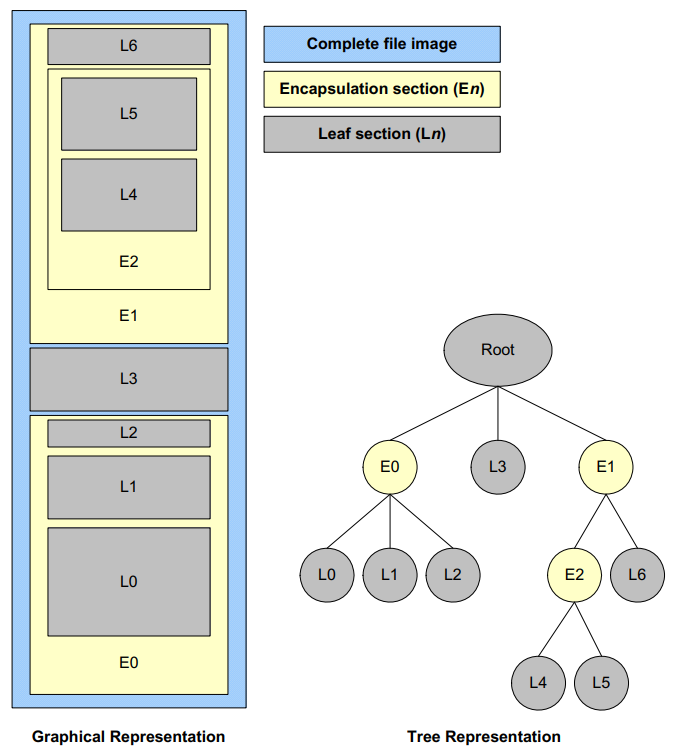
\includegraphics[width=\linewidth]{architecture/firmware-file-system-representation}
	\caption{Example File System Image}\label{fig:architecture-firmware-file-system-representation}
\end{figure}

In the example shown in Figure \ref{fig:architecture-firmware-file-system-representation}, the file image root contains two encapsulation sections (E0 and E1) and one leaf section (L3). The first encapsulation section (E0) contains children, all of which are leaves (L0, L1, and L2). The second encapsulation section (E1) contains two children, one that is an
encapsulation (E2) and the other that is a leaf (L6). The last encapsulation section (E2) has two children that are both leaves (L4 and L5)


